%!TEX root = ../thesis.tex

\chapter{引言}

\section{我国信用债违约回顾}

过去一段时间,我国信用债市场维持着“刚兑”神话,而自 2014 年“11 超日债”违约以来,我国信用债市场中投资者“刚性兑付”的“信仰”逐步动摇、破灭。及至 2021 年,永城煤电、华晨宝马的违约打破了人们对 AAA 级国企的“刚兑信仰”,恒大、海航违约使人们意识到并不存在所谓“大而不倒”。近年来一些典型的债券违约事件如表\ref{tab:defaults_in_history}所示。

\begin{table}[ht]
	\caption{近年来部分影响较大的违约事件}
	\centering
	\begin{tabular}{lccc}
		债券名称         & 违约日期   & 原因               & 影响                   \\ \hline
		11超日债         & 2014-03-05 & 过度扩张资金链断裂 & 打破刚兑的开始         \\
		11天威MTN2       & 2015-04-21 & 经营亏损资不抵债   & 打破国企刚兑           \\
		14波鸿CP001      & 2015-04-12 & “技术性”违约       & 首例“技术性违约”       \\
		15五洋债         & 2018-08-16 & 欺诈发行           & 首例公司债券欺诈发行案 \\
		16民生投资PPN001 & 2019-01-29 & “技术性”违约       & AAA 债券违约第一例     \\
		20永煤SCP003     & 2020-11-26 & 逃废债             & 河南全省融资环境恶化   \\
		15天安人寿       & 2020-12-29 & 股东抽血           & 金融机构破刚兑付       \\
		17幸福基业MTN001 & 2021-02-27 & 过度扩张遇宏观调控 & 地产债违约潮的开始     \\
	\end{tabular}
	\label{tab:defaults_in_history}
\end{table}
事实上,“刚兑”并非正常现象,反而容易导致风险的无序累积。在经济周期的起伏过程中,企业经营失败不可避免。通过违约释放部分信用风险,反而能降低大规模系统性金融风险发生的概率。违约可以使泡沫膨胀到更大前提前破裂,如近期的房地产企业的加速出清,就是过去房企高杠杆经营扩张的反噬。如果长时间维持高杠杆经营,居民部门负债率高企,地产商开发贷终将难以维续,势必会对银行系统造成很大的威胁,进而影响我国金融稳定。

然而,债务违约毕竟会带来多方面的危害。对投资人来说,投资失败意味着不小的损失;对发行人则意味着丧失外部融资功能、经营难以维系。此外,违约还有一定的外部性,如果处理不好,如永煤逃废债,则可能会影响区域乃至全国的投融资环境,进而会对整个经济体造成影响。这些企业违约的原因各有不同,主要包括:技术原因场外兑付(如中融新大),评级公司下调评级(如花样年、新力),公司流动性遇到了暂时的困难(如恒大)等。因此,如何准确评估企业违约风险,使得各方利益相关者在违约事件出现之前有所准备,是一个重要问题。

\begin{figure}[ht]
	\centering
	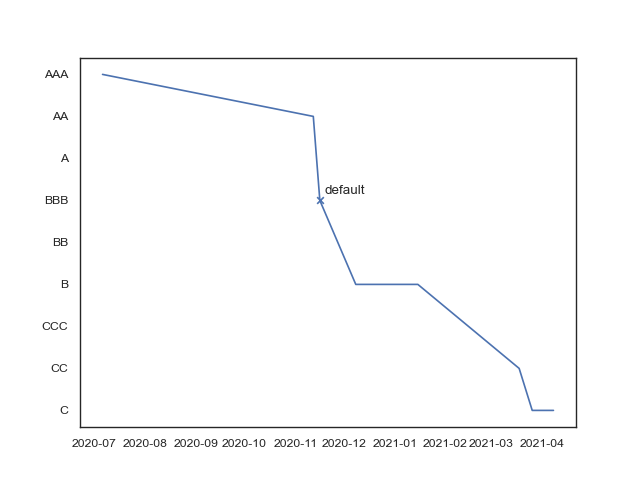
\includegraphics[width=0.9\linewidth]{./data/rating_of_zg.png}
	\caption{某评级公司对某违约发行人的历史评级}
	\label{fig:rating_of_zg}
\end{figure}
评级是债券信用风险评估的常用工具,是判断公司违约风险最直观的手段,但信用评级却屡屡失灵。例如,有些评级机构为了维护发行人利益,初始时给予某债券很高的评级,随后在违约事件已经板上钉钉的情况下,几天内连续下调原先的虚高评级至垃圾级,如图\ref{fig:rating}所示的某违约企业评级历史。又如,被\Textcite{王雄元2013声誉机制}列为低声誉评级机构的大公国际,因涉嫌帮助欺诈发行“五洋债”,应承担 10\% 的连带责任赔偿 7400 万元。但大公竟称“公司已经发不出工资,顶多赔偿 150 万元”,最终被列入失信被执行人,可见某些评级机构对自身声誉的重视程度。因此,本文试图从微观、中观和宏观三个层面出发,对企业债券违约的影响因素进行分析,探讨对债券违约风险进行全面客观评价的模型。

本文主要内容如下:第一章回顾并梳理现有的有关研究;第二章基于理论和实践归纳违约的影响因素;第三章分别基于计量和机器学习手段进行了研究设计,第四章对理论进行实证检验,第五章进行了稳健性检验;第六章对全文进行总结。
\section{文献综述}
\label{sec:zs}
在信用评级质量方面,很多研究发现,评级机构的利益动机会对评级质量产生影响。评级机构在行业竞争的情况下,为了获得收入,会对公司虚高评级,即使是国际著名的评级机构也无法避免\cite{opp2013rating}。甚至在违约发生后,涉事评级机构非但不考虑模型是否有偏误,反而为了争取市场份额而放宽标准,以提高评级\cite{黄小琳2017债券违约对涉事信用评级机构的影响}。此外,付费模式也会使得评级机构失去独立性,在“发行人付费”模式下,信用评级虽然可以在一定程度上包含公司的内部私有信息,但由于独立性缺失,其总体的信用评级质量仍然低于“投资人付费”模式下的信用评级质量,使得部分评级机构声誉较差\cite{吴育辉2020,陈关亭2021多重信用评级与债券融资成本}。因此,评级可能并不是一种有效的信用评估方式 \cite{blochlinger2018ratings}。

除评级之外,学者们还从不同层面讨论了违约的影响因素。

在公司层面,对违约的讨论主要基于公司治理。\Textcite{林晚发2018高管任职经历的得与失}从高管任职经历出发,发现有高管担任过人大代表或政协委员的企业债券发行成功率更高,\Textcite{anginer2018corporate}提出一个涵盖管理、约束、独立三方面指标的公司治理指标,并指出公司治理增加一个标准差使银行的违约距离指标降低了 0.14 个标准差。\Textcite{ding2021corporate}和\Textcite{subrahmanyam2017credit}分别从疫情和引入 CDS 对公司治理的影响出发, 研究外生冲击由于公司治理能力的差异影响偿债能力的差异。

在市场层面,有学者从市场信号的角度研究违约。有些是直接研究信用债的利差,如\Textcite{纪志宏2017信用风险溢价还是市场流动性溢价}利用跨市场债的利差分析流动性和信用风险分别对利差的贡献。也有些是利用信用衍生品的数据,如\Textcite{bonaccolto2021breakup}利用 CDS ,研究疫情对欧盟成员国债券违约风险的冲击。经典的信用风险模型如莫顿模型、KMV 模型等亦是利用市场价格信号预测违约的,但是这些理论在实践中系统性地低估了实际投资级债券信用利差的水平,即所谓“信用利差之谜”,\Textcite{feldhutter2018myth}认为源于莫顿模型的不正确应用,而\Textcite{bai2020credit}则持相反观点,认为是巨大的市场风险价格归因于具有重大下行尾部风险敞口的证券,标准的基于扩散的违约结构模型被错误指定,因而模型显著低估了短期信用利差。

在宏观层面,\Textcite{bai2019common} 和\Textcite{bali2021macroeconomic}分别从宏观经济下行和宏观经济不确定性出发,研究宏观环境对于公司债利差的影响。宏观政策角度,\Textcite{王博2019货币政策不确定性}指出货币政策不确定性的增加会带来违约风险的上升。\Textcite{梅冬州2021财政扩张} 和\Textcite{2020Fiscal} 则认为财政扩张导致挤出效应,从而民企面临融资困境,进而违约率上升,利差走阔。此外,流动性可能会影响违约\cite{brogaard2017stock},更高的流动性可以通过提高价格效率来降低违约风险,或者通过放松投资者的退出能力来改善公司治理。

在风险传染方面,有关研究主要集中在系统性风险传染。\Textcite{苟文均2016债务杠杆与系统性风险传染机制}基于 CCA 模型,提出杠杆率应从较高居民转移至政府等低杠杆部门,以降低违约风险。
\Textcite{2020Do}基于 VaR 模型,认为几乎所有的系统性风险指标对对违约率都有预测能力。
非系统性风险方面,\Textcite{azizpour2018exploring}认为公司之间的财务、法律或业务关系可能充当风险分散的渠道,通过捕捉系统性风险和这种非系统性的聚类,可以几乎完美地匹配了的时间变化结果所隐含的时间变化的违约计数和违约时间的理论分布。

综上,现有文献较为分散地分析单方面影响违约的因素,少有揭示违约因素间的相互作用,且对我国目前债券市场上风险逐步释放的现状估计不足。因此,本文聚焦于将不同违约因素进行整合,采用自下而上的方式,归纳违约因素,比较违约因素之间的相对重要性,并通过决策树、随机森林等算法刻画违约因素之间的相互作用。
本文的贡献在于:结合理论与实务中的新现象,系统性整理了违约因素,并采用机器学习算法探究违约因素间的相互作用。
